\chapter{Computational Fluid Structure Interaction}

The multi-disciplinary nature of computational fluid-structure interaction , involves addressing issues regarding computational fluid dynamics and computational structure dynamics. In general, CFD and CSM are individually well-studied, in terms of numerical solution strategies. CFSI adds another layer of complexity to the solution process, (1) the \textit{coupling} of the fluid and solid equations , (2) the tracking of \textit{interface} separating the fluid and solid domains. The coupling pose two new conditions at the interface absent from the original fluid and solid conditions, which is \textit{continuity of velocity} and \textit{continuity of stress} at the interface.

\begin{align}
\mathbf{v}_f = \mathbf{v}_s \\
\mathbf{\sigma}_f \cdot \mathbf{n} = \mathbf{\sigma}_s \cdot \mathbf{n}
\end{align}


The tracking of the interface is a issue, due to the different description of motion used in the fluid and solid problem. If the natural coordinate system are used for the fluid problem and solid problem, namely the eulerian and lagrangian description of motion, the domains doesn't match and the interface. Tracking the interface is aslo essential for fulfilling the interface boundary conditions. As such only one of the domains can be described in its natural coordinate system, while the other domain needs to be defined in some transformed coordinate system.   \\ 

Fluid-structure interaction problems are formally divided into the \textit{monolithic} and \textit{partitioned} frameworks.  In the monolithic framework, the fluid and solid equations together with interface conditions are solved simultaneously. The monolithic approach has the advantage of fullfilling the \textit{kinematic} (1.1) and \textit{dynamic}(1.2) interface conditions with high accuracy. The method is then said to be \textit{strongly coupled}. However, the complexity of solving all the equations simuntainiously and the strong coupling contributes to a stronger nonlinear behaviour of the whole system \cite{Wick}. The complexity also makes monolithic implementations \textit{ad hoc} and less modular, and the nonlinearity makes solution time slow.

In the \textit{partitioned} framework one solves the equations of fluid and structure subsequently. Sovling the fluid and solid problems individually is beneficial, in terms of the wide range of optimized solvers and solution strategies developed for each sub-problem. A major drawback is the methods ability to enfore the \textit{kinematic} (1.1) and \textit{dynamic}(1.2) conditions at each timestep. Therefore partitioned solution strategies are defined as  \textit{weakly} coupled. However, by sub-iterations between each sub-problem at each timestep, (1.1) and (1.2) can be enforced with high accuracy, at the cost of increased compuational time. For some applications, low-accuracy of the interface conditions are suffictient such as aeroelasticity \cite{Fernandez2009}. \\

Capturing the interface is matter of its own, regardless of the the monolithic and partitioned frameworks.
The scope of interface methods are divided into \textit{interface-tracking} and \textit{interface-capturing } methods.\cite{Frei2016}. In the \textit{Interface-tracking} method, the mesh moves to accommodate for the movement of the structure as it deformes the spatial domain occupied by the fluid. As such, the mesh itself "tracks" the fluid-structure interface as the domain undergoes deformation. Interface-capturing yields better control of mesh resolution near the interface, which in turn yeilds better control of this critical area in terms of enforcing the interface conditions.
However, moving the mesh-nodes pose potential problems for mesh-entanglements, restricting the possible extent of deformations.  

In \textit{interface-capturing} methods one distinguish the fluid and solid domains by some phase variable over a fixed mesh, not resolved by the mesh iteself. This approach is in general not limitied in terms of deformations, but suffers from reduced accuracy at the interface. \cite{Frei2016}. 

\begin{figure}[h!]
  \centering
    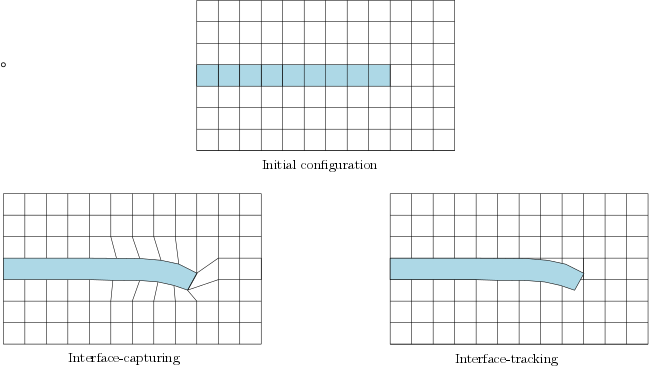
\includegraphics[scale=0.5]{./Fig/interface.png}
      \caption{Comparison of interface-tracking and interface-capturing for an elastic beam undergoing deformation}
\end{figure}

Among the multiple approaches within CFSI, the arbitary Lagrangia-Eulerian methos is chosen for this thesis. 



%We define $\Omega$ in the \textit{reference configuration} be partitioned in a fluid domain $\hat{\Omega_f}$ and a structure domain $\hat{\Omega_s}$ such that
%$\Omega = \hat{\Omega_f} \cup \hat{\Omega_s}$. Further we define the interface $\hat{\Gamma}$ as the interface between these domains such that $\Gamma_i = \hat{\partial \Omega_f} \cap \hat{\partial %\Omega_s}$. 
%The fluid-structure interaction problem is then defined by the fluid and solid equations, and the transmission of the \textit{kinematic} and \textit{dynamic} conditions on the interface $\hat{\Gamma}$. 


%\section{Fully Eulerian}
%This method keeps the fluid in its \textit{Eulerian coordinates}, and such can be seen as the natural counterpart of the ALE method \cite{Wick2013}. First proposed by , \cite{Dunne2006}. One motivation of such and approach is the handling of large-deformation, as the transformation to eulerian coordinates are purely natural.

\section{Arbitary Lagrangian Eulerian formulation}
The \textit{arbitary Lagrangian-Eulerian} formulation is the most popular approach within \textit{Interface-tracking} \cite{Richter2010a}, \cite{Frei2016}, initially developed to combine the strengths of the \textit{Lagranngian} and \textit{Eulerian} coordinate systems. In this approach the structure is given in its natural \textit{Lagrangian coordinate system}, while transforming the fluid domain into an artificial coordinate system similar to the \textit{Lagrangian coordinate system}. Since no natural displacement occur in the fluid domain, the transformation has no directly physical meaning \cite{Richter2010a}, \cite{Donea2004}. 
 
With this in mind, we will derive these transformations with the help of a new arbitary fixed reference system \ha{W}, following the ideas and approaches found in \cite{Richter2016}. Further we denote its deformation gradient as $\hat{F}_w$ and its determinant $\ha{J}_w$. Following the ideas from chapter 2, we introduce the invertibale mapping $\ha{T}_w : \ha{W} \rightarrow V(t)$ , with the scalar $\ha{f}(\ha{x}_W, t) = f(x,t) $ and vector $\hat{w}(\ha{x}_W, t) = \mathbf{w}(x,t) $ counterparts.\\ 
For $\ha{V} = \ha{W}$, $\ha{W}$ simply denotes the familiar Lagrangian description.
In the case $\ha{V} \neq \ha{W}$, $\ha{W}$ as pointed out earlier have no direct physical meaning.  Hence it is important to notice that the physical velocity $\hat{v}$ and the velocity of arbitrary domain $\pder{\ha{W}_w}{t}$ doesn't necessary coincide. This observation is essential, as we will soon see. \\

We will first define the transformation of spatial and temporal derivatives from $V(t)$ to $\ha{W}$ found in \cite{Richter2016}\\

\begin{lem}
Transformation of scalar spatial derivatives \\
\textit{Let f be a scalar function such that} $f: V(t) \rightarrow \mathbb{R}$, \textit{then} 
\begin{align}
\nabla f = \hat{F}_W^{-T} \hat{\nabla}\ha{f}
\end{align} 
\end{lem}

\begin{lem}
Transformation of vector spatial derivatives \\
\textit{Let \textbf{w} be a vector field such that} $\mathbf{w}: V(t) \rightarrow \mathbb{R}^d$, \textit{then} 
\begin{align}
\nabla \mathbf{w} = \hat{\nabla}\hat{w} \hat{F}_W^{-1} 
\end{align} 
\end{lem}

\begin{lem}
Transformation of scalar temporal derivatives \\
\textit{Let f be a scalar function such that} $f: V(t) \rightarrow \mathbb{R}$, \textit{then} 
\begin{align}
\pder{f}{t} = \pder{\ha{f} }{t} - (\hat{F}_W^{-1} \pder{\ha{T}_W}{t} \cdot \hat{\nabla}) \ha{f}
\end{align} 
\end{lem}

In addition we need a consistent way to transform the induced stresses in the \textit{Eulerian} coordinate system to $\ha{W}$. Hence we introduce the \textit{Piloa transformation}, found in most introduction courses in structure mechanics.
\\
\begin{lem}
T \\
\textit{Let \textbf{w} be a vector field such that} $\mathbf{w}: V(t) \rightarrow \mathbb{R}^d$, \textit{then the Piola transformation of w is defined by} 
\begin{align}
\mathbf{w} = \ha{J}_W \hat{F}^{-1}_W \hat{w}
\end{align} 
\end{lem}

The Piola transformation can be further extended to transform tensors, see \cite{Richter2016}, Orange book. This results is essential as it allows us to transform surface forces induced by the \textit{Cauchy stress tensor} on our arbitrary coordinate system $\ha{W}$. Lemma 1.4 brings us to \textit{the first Piola Kirchhoff stress tensor} $\hat{P} = \ha{J}_W \hat{\sigma}\hat{F}_W^{-T}$.

\subsection{ALE formulation of the fluid problem}

Recall the Navier-Stokes equation defined in the \textit{Eulerian coordinate system} V(t).
\begin{align*}
&\rho \pder{\mathbf{v}}{t} + \rho \mathbf{v} \cdot \nabla \mathbf{v} =
\nabla \cdot \sigma + \rho \mathbf{f} \\
&\nabla \cdot \mathbf{v} = 0
\end{align*}
Using our newly introduced transformations of derivatives we map the equation to the arbitrary reference system $\ha{W}$. We will first consider the transformation of the\textit{material derivative}. By 
\begin{align*}
\frac{d \mathbf{v}}{dt}(x,t) = \pder{\mathbf{v}}{t}(x,t) + \nabla \mathbf{v}(x,t) \cdot \pder{x}{t} \\
\frac{d \mathbf{v}}{dt}(x,t) = \pder{\mathbf{v}}{t}(x,t) + \nabla \mathbf{v}(x,t) \cdot \mathbf{v}
\end{align*}
Note $\pder{x}{t}$ is the velocity of particles and not the transformation velocity $\pder{\ha{T}_W}{t}$. By lemma(1.1, 1.2, 1.3) we have  

\begin{align*}
\frac{d \mathbf{v}}{dt}(x,t) = 
\pder{\hat{v}}{t}(x,t) - (\hat{F}_W^{-1}\pder{\ha{T}_W}{t} \cdot \hat{\nabla})\hat{v}
+ \hat{F}_W^{-T}\hat{\nabla}\hat{v} \cdot \hat{v} \\
\mathbf{v} \cdot \nabla \mathbf{v} = \nabla \mathbf{v} \mathbf{v} = 
\hat{\nabla}\hat{v}\hat{F}_W^{-1}\hat{v} = (\hat{F}_W^{-1}\hat{v} \cdot \hat{\nabla})\hat{v} \hspace{4mm} \textit{FINN KILDE}
\end{align*}

These results can be used to show that

\begin{align*}
\pder{\mathbf{v}}{t} + \mathbf{v} \cdot \nabla \mathbf{v} =
\pder{\hat{v}}{t} + (\hat{F}_W^{-1}(\hat{v} - \pder{\ha{T}_W}{t}) \cdot \hat{\nabla}) \hat{v}
\end{align*}

By applying \textit{the first Piola Kirchhoff stress tensor} directly we transform the surface stress by 

\begin{align*}
\nabla \cdot \sigma = \nabla \cdot (\ha{J}_W \hat{\sigma}\hat{F}_W^{-T})
\end{align*}
In general, $\sigma$ is presumed on the form of a Newtonian fluid.
However special care must be taken, as $\sigma \neq \hat{\sigma}$ due to spatial derivatives within the tensor. Hence 
\begin{align*}
\sigma = -p I + \mu_f(\nabla \mathbf{v} + (\nabla \mathbf{v})^T \\
\hat{\sigma} = -\ha{p} I + \mu_f(\hat{\nabla}\hat{v}\hat{F}_W^{-1} +\hat{F}_W^{-T}\hat{\nabla}\hat{v}^T )
\end{align*} 

For the conservation of continuum we apply the \textit{Piola Transformation} such that

\begin{align*}
\nabla \cdot \mathbf{v} = \nabla \cdot (\ha{J} \hat{F}_W^{-1} \hat{v})
\end{align*}

\subsection{ALE formulation of the solid problem}

With the introduced mapping identities we have the necessary tools to derive a full fluid-structure interaction problem defined of a fixed domain. Since the structure already is defined in its natural Lagrangian coordinate system, no further derivations are needed for defining the total problem.

\begin{equat}
\textit{ALE problem on a fixed domain}
\begin{align}
\ha{J} \pder{\hat{v}}{t} + \ha{J} (\hat{F}_W^{-1}(\hat{v} - \pder{\ha{T}_W}{t}) \cdot \hat{\nabla}) \hat{v}
= \nabla \cdot (\ha{J}_W \hat{\sigma}\hat{F}_W^{-T}) + \rho_f \ha{J} \mathbf{f}_f
\hspace{4mm} \text{in} \hspace{2mm} \Omega_f \\
\nabla \cdot (\ha{J} \hat{F}_W^{-1} \hat{v}) \hspace{4mm} \text{in} \hspace{2mm} \Omega_f \\
\rho_s \pder{\hat{v}_s}{t} = \nabla \cdot \mathbf{F}\mathbf{S} + \rho_s \mathbf{f}_s
\hspace{4mm} \text{in} \hspace{2mm} \Omega_s \\
\pder{\hat{v}_s}{t} = \hat{u}_s \hspace{4mm} \text{in} \hspace{2mm} \Omega_s \\
\hat{v}_s = \hat{v}_f \hspace{4mm} \text{on} \hspace{2mm} \Gamma_i \\
\ha{J}_W \hat{\sigma}\hat{F}_W^{-T} \cdot \mathbf{n} = 
\mathbf{F}\mathbf{S} \cdot \mathbf{n}  \hspace{4mm} \text{on} \hspace{2mm} \Gamma_i 
\end{align}
\end{equat}


\subsection*{Fluid mesh movement}
In the ALE framwork one of the most limiting factors is the degeneration of the mesh due to large deformations. Even the most advanced ALE formulated schemes reaches a limit when only re-meshing is nesecarry \cite{Wall12006}. Consequently the choice of an appropriate mesh moving technique is essential to preserve a feasible mesh quality for the simulation of fluid flow. Let the total domain deformation $\ha{T}(\ha{x}, t)$ be divided into the solid and fluid deformation $T_s$, $T_f$, were the fluid deformation is mapped to the arbitrary fixed reference system $\ha{W}$ presented in the last subsection.  
Then the ALE map $T_f$ on the form 
\begin{align*}
\ha{T}_f(\ha{x}, t) = \hat{x} + \hat{u}_f(\hat{x}, t)
\end{align*}
is constructed such that $\hat{u}_f$ is an extension of the solid deformation $\hat{u}_s$ from the interface to the fluid domain. Several extentions have been proposed throuhout the litteratur, and for an overview the reader is refered to \cite{MM2016}, and the reference therein. The construction of such extensions often involves solving some auxiliary problem on a partial differential equation(PDE) form, mainly of second-order. The \textit{Laplacian} and \textit{pseudo-elasticity} extentions are examples, which will be considered in this thesis. These extensions are beneficial in terms of simplicity and computational efficiency, but comes with a cost of user mesh customization. One often want to ensure a desired mesh position and some regularity of mesh spacing on the boundary, but it is impossible for second order extensions to specify both \cite{Helenbrook2003}. Therefore the author of \cite{Helenbrook2003}, proposes a fourth-order PDE, the \textit{biharmonic} extensions, to improve the regularity of the mesh deformation. \\

\subsubsection*{Laplacian model}

The main motivation for a \textit{Laplacian} smoothing is due to its simplicity and due to its property of bounding the interior displacements to the boundary values. 

\begin{align*}
&- \hat{\nabla} \cdot (\alpha^q \hat{\nabla} \hat{u}) = 0 \\
&\hat{u}_f = \hat{u}_s \hspace{2mm} \text{on} \hspace{2mm}  \Gamma \\
&\hat{u}_f = 0 \hspace{2mm} \text{on} \hspace{2mm} \partial \hat{\Omega}_f / \Gamma 
\end{align*}

Most favourable, the largest mesh deformation occuring should be confined to the interal part of the mesh as it causes the least distortion \cite{Jasak2006}. Therefore the introduced diffusion parameter $\alpha$, often raised to some power q, is introduced to manipulate this behaviour. The form of this paramter is often problem specific,  as selective treatment of the elements may vary from different mesh deformation problems. A jacobian based method was introduced in \cite{Stein}. In \cite{Jasak2006}, the authors reviewed several distance based options, where $\alpha$ was some function of the distance to the closest moving boundary. This method was adopted in this thesis on the form

\begin{align*}
\alpha(x) = \frac{1}{x^q}  \hspace{4mm} q = -1
\end{align*}

However as pointed out by \cite{Hsu}, one of the main disadvantages of using the linear Laplace equation is that the equation solves the mesh deformation components independently of one another. Say one have deformation only in the x-coordinate direction, the interior mesh points will only be moved along this deformation. Such a behavior restricts the use to the Laplace equation of mesh extrapolation purposes.

\subsubsection*{Linear elastic model}
Considering a linear elastic model for mesh moving was first introduced in \cite{Tezduyar1992}.  
Both \cite{Dwight}
\begin{align*}
&\nabla \cdot \sigma = 0 \\
&\sigma = \lambda Tr(\epsilon(u)) I + 2 \mu \epsilon(u) \\
&\epsilon(u) = \frac{1}{2}(\nabla u + \nabla  u^T)
\end{align*}

Where Lamé constants $\lambda$ and $\nu$ are given as

\begin{align*}
\lambda = \frac{\nu E}{(1 + \nu)(1 - 2\nu)} \hspace{2mm} \mu = \frac{E}{2(1 + \nu)}
\end{align*}

One of the main motivations for introducing such a model is the manipulation of Young's modulus $E$, and the poisson´s ration $\nu$. Recall that Young's modulus is the measurement of the a materials stiffness, while the poission's ratio describe the materials stretching in the transverse direction under extension in the axial direction. Manipulating these parameters one can influence the mesh deformation,
however the choice of these parameters have proven not to be consistent,  and to be dependent of the given problem.  \\

In \cite{Wicka} the author proposed a negative possion ratio, which makes the model mimic an auxetic material. Such materials becomes thinner in the perpendicular direction when they are submitted to compression, and this property is feasible for mesh under deformation. 

One of the most common approach is to set $\nu$ as a constant in the range $\nu \in [0, 0.5)$ and let $E$ be the inverse of the distance of an interior node to the nearest boundary surface \cite{MM2016}. 
The authors of \cite{Biedron} used this property and also argued that the Young's modulus also could be chosen as the inversely proportional to the cell volume. They also pointed out that both approaches would give the desired result that the small cells around the solid surface would modeled rigid, moving with the surface of the solid as it undergoes deformation. On the other hand cells further away will deform to counter the effects close to the solid surface.

\subsubsection*{Biharmonic model}
Using a biharmonic mesh deformation model provides further freedom in terms of boundary conditions, and the reader is encoured to consult \cite{Helenbrook2003} for a deeper review. We will in combination with \cite{Wicka} present two main approaches the biharmonic model is defined as 
\begin{align*}
\hat{\nabla}^2 \ha{u} = 0 \hspace{4mm} \text{on} \hspace{2mm} \hat{\Omega}_f 
\end{align*}
By introducing a second variable on the form $\ha{w} = - \hat{\nabla} \ha{u}$, we get the following system defined by 
\begin{align*}
&\hat{w} = -\hat{\nabla}^2\hat{u} \\
&- \hat{\nabla} \hat{w} = 0
\end{align*}

This model is defined in a mixed formulation, and as such the prize for quality and control of mesh deformation comes with the cost of more computational demanding problem. 

For the boundary conditions two types has been proposed in \cite{Wicka}. Let 
$\hat{u}_f$ be decomposed by the components $\hat{u}_f = (\ha{u}_f^{(1)}. \ha{u}_f^{(2)})$. Then we have

\begin{align*}
&\textbf{Type 1} \hspace{4mm} \ha{u}_f^{(k)} = \pder{\ha{u}_f^{(k)}}{n} = 0 \hspace{4mm} \partial \hat{\Omega}_f / \Gamma \hspace{2mm} \text{for} \hspace{1mm} k = 1, 2 \\
&\textbf{Type 2} \hspace{4mm} \ha{u}_f^{(1)} = \pder{\ha{u}_f^{(1)}}{n} = 0 
\hspace{2mm} \text{and} \hspace{2mm} \ha{w}_f^{(1)} = \pder{\ha{w}_f^{(1)}}{n} = 0 \hspace{4mm} \text{on} \hspace{1mm} \hat{\Omega}_f^{in} \cup \hat{\Omega}_f^{out} \\ 
&\hspace{17mm}  \ha{u}_f^{(2)} = \pder{\ha{u}_f^{(2)}}{n} = 0 
\hspace{2mm} \text{and} \hspace{2mm} \ha{w}_f^{(2)} = \pder{\ha{w}_f^{(2)}}{n} = 0 \hspace{4mm} \text{on} \hspace{1mm}  \hat{\Omega}_f^{wall}
\end{align*}

With the first type of boundary condition the model can interpreted as the bending of a thin plate, clamped along its boundaries. The form of this problem has been known since 1811, and its derivation has been connected with names like  French scientists Lagrange, Sophie Germain, Navier and Poisson \cite{Meleshko1997}.  

The main motivation for second type of boundary condition is for a rectangular domain where the coordinate axes match the Cartesian coordinate system \cite{Wicka}. In such a configuration, the mesh movement is only constrained in the perpendicular direction of the fluid boundary, leading to mesh movement in the tangential direction. This special case reduces the effect of distortion of the cells.  

\newpage

\newpage
\section{Discretization of the FSI problem}
Say something general of FSI discretization.. FEM, FVM, ...
In this thesis, the finite element method will be used to discretize the coupled fluid-structure interaction problem. It is beyound of scope  of this thesis, to thorough dive into the analysis of the finite element method regarding fluid-structure interaction problems. Only the basics of the method, which is nesecarry in order to define a foundation for problem solving will be introduced. 

\subsection{Finite Element method}
Let the domain $\Omega(t) \subset \mathbb{R}^d \ (d = 1, 2, 3) $  be a time dependent domain discretized a by finite number of d-dimentional simplexes.  Each simplex is denoted as a finite element, and the union of these elements forms a mesh. Further, let the domain be divided by two time dependent subdomains $\Omega_f$ and $\Omega_s$, with the interface $\Gamma = \partial \Omega_f \cap \partial \Omega_s$. The initial configuration $\Omega(t), t = 0 $ is defined as $\hat{\Omega}$, defined in the same manner as the time-dependent domain. $\hat{\Omega}$ is  known as the \textit{reference configuration}, and hat symbol will refer any property or variable to this domain unless specified. The outer boundary is set by $\partial \hat{\Omega}$ , with $\partial \hat{\Omega}^D$ and $\partial \hat{\Omega}^N$ as the Dirichelt and Neumann boundaries respectively. \\ \\

The family of Lagrangian finite elements are chosen, with the function space notation,
\begin{align*}
\hat{V}_{\Omega} := H^1(\Omega) \hspace{4mm} 
\hat{V}_{\Omega}^0 := H_0^1(\Omega)  
\end{align*}
where $H^n$ is the Hilbert space of degree n. \\
Let Problem 2.1 denote the strong formulation. By the introduction of appropiate trial and test spaces of our variables of interest, the weak formulation can be deduced by multiplying the strong form with a test function and taking integration by parts over the domain.  This reduces the differential equation of interest down to a system of linear equations. (skriv bedre..) \\
The velocity variable is continous through the solid and fluid domain
\begin{align*}
\hat{V}_{\Omega, \gat{v}} := \gat{v} \in H_0^1(\Omega), \hspace{2mm} 
\gat{v}_f = \gat{v}_s \ \text{on} \ \hat{\Gamma}_i \\
\hat{V}_{\Omega, \gat{\psi}} := \gat{\psi}^u \in H_0^1(\Omega), \hspace{2mm} 
\gat{v}_f = \gat{v}_s \ \text{on} \ \hat{\Gamma}_i 
\end{align*}
For the deformation, and the artificial deformation in the fluid domain let
\begin{align*}
\hat{V}_{\Omega, \gat{v}} := \gat{u} \in H_0^1(\Omega), \hspace{2mm} 
\gat{u}_f = \gat{u}_s \ \text{on} \ \hat{\Gamma}_i \\
\hat{V}_{\Omega, \gat{\psi}} := \gat{\psi}^v \in H_0^1(\Omega), \hspace{2mm} 
\gat{\psi}_f^v = \gat{\psi}_s^v \ \text{on} \ \hat{\Gamma}_i 
\end{align*}

For simplification of notation the inner product is defined as
\begin{align*}
\int_{\Omega} \gat{v} \ \gat{\psi} \ dx = (\gat{v}, \ \gat{\psi})_{\Omega}
\end{align*}
 

\subsection{Variational Formulation}
With the primaries set, we can finally define the discretization of the monolithic coupled fluid-structure interaction problem. For full transparency, variation formulation of all previous suggested mesh motion models will be shown. For brevity, the laplacian and linear elastic model will be shorted such that 
\begin{align*}
&\hat{\sigma}_{\text{mesh}} = \alpha \nabla \mathbf{u} \hspace{2mm} \text{Laplace} \\
&\hat{\sigma}_{\text{mesh}} =  \lambda Tr(\epsilon(\mathbf{u})) I + 2 \mu \epsilon(\mathbf{u}) \hspace{2mm} \text{Linear Elasticity} 
\end{align*}
Further, only the biharmonic model for the first type of boundary condition will be introduced as the second boundary condition is on a similar form.
  By the concepts of the Finite-element method, the weak variation problem yields.

\begin{prob}
\textit{Coupled fluid structure interaction problem for laplace and elastic mesh moving model.
Find $\bat{u}_s, \bat{u}_f, \bat{v}_s, \bat{v}_f, \ha{p}_f $ such that}
\begin{align*}
\big(\ha{J} \pder{\bat{v}}{t}, \ \gat{\psi}^u \big)_{\hat{\Omega}_f} +
\femf{\ha{J} (\hat{F}_W^{-1}(\bat{v} - \pder{\ha{T}_W}{t}) \cdot \hat{\nabla}) \bat{v}}{\gat{\psi}^u}
+ \femi{\ha{J}_W \hat{\sigma}\hat{F}_W^{-T} \bat{n}_f}{\gat{\psi}^u} \\
- \femf{\ha{J}_W \hat{\sigma}\hat{F}_W^{-T}}{\hat{\nabla}\gat{\psi}^u} -
\femf{\rho_f \ha{J} \mathbf{f}_f}{{\gat{\psi}^u}} = 0 \\
\fems{\rho_s \pder{\bat{v}_s}{t}}{\gat{\psi}^u} + \femi{\bat{F}\bat{S}\bat{n}_f}{\gat{\psi}^u}
- \fems{\bat{F}\bat{S}}{\nabla \gat{\psi}^u} - \fems{\rho_s \bat{f}_s}{\gat{\psi}^u} = 0 \\
\fems{\pder{\bat{v}_s - \bat{u}_s}{t}}{\gat{\psi}^v}  = 0\\
\femf{\nabla \cdot (\ha{J} \hat{F}_W^{-1} \bat{v})}{\gat{\psi}^p} = 0 \\
\femf{\hat{\sigma}_{\text{mesh}}}{\hat{\nabla}\gat{\psi}^u} = 0
\end{align*} 
\end{prob}

\begin{prob}
\textit{Coupled fluid structure interaction problem for biharmonic mesh moving model.
Find $\bat{u}_s, \bat{u}_f, \bat{v}_s, \bat{v}_f, \ha{p}_f $ such that}
\begin{align*}
\big(\ha{J} \pder{\bat{v}}{t}, \ \gat{\psi}^u \big)_{\hat{\Omega}_f} +
\femf{\ha{J} (\hat{F}_W^{-1}(\bat{v} - \pder{\ha{T}_W}{t}) \cdot \hat{\nabla}) \bat{v}}
{\gat{\psi}^u}
+ \femi{\ha{J}_W \hat{\sigma}\hat{F}_W^{-T} \bat{n}_f}{\gat{\psi}^u} \\
- \femf{\ha{J}_W \hat{\sigma}\hat{F}_W^{-T}}{\hat{\nabla}\gat{\psi}^u} -
\femf{\rho_f \ha{J} \mathbf{f}_f}{{\gat{\psi}^u}} = 0 \\
\fems{\rho_s \pder{\bat{v}_s}{t}}{\gat{\psi}^u} + \femi{\bat{F}\bat{S}\bat{n}_f}{\gat{\psi}^u}
- \fems{\bat{F}\bat{S}}{\nabla \gat{\psi}^u} - \fems{\rho_s \bat{f}_s}{\gat{\psi}^u} = 0 \\
\fems{\pder{\bat{v}_s - \bat{u}_s}{t}}{\gat{\psi}^v}  = 0\\
\femf{\nabla \cdot (\ha{J} \hat{F}_W^{-1} \bat{v})}{\gat{\psi}^p} = 0 \\
\femf{\hat{\nabla}\bat{u}}{\hat{\nabla}\gat{\psi}^{\eta}} - 
\femf{\bat{w}}{\hat{\nabla}\gat{\psi}^u} = 0 \\
\femf{\hat{\nabla}\bat{w}}{\hat{\nabla}\gat{\psi}^{v}} = 0
\end{align*}
\text{for the first type of boundary conditions introduced. } 
\end{prob}

Both problems introduced must handle the \textit{kinematic} and \textit{dynamic} boundary conditions in a consistent way. By a continuous velocity field on the whole domain, the \textit{kinematic} condition is strongly enforces on the interface $\hat{\Gamma}_i$
The continuity of normal stresses on the interface are defined as
\begin{align*}
 \femf{\ha{J}_W \hat{\sigma}\hat{F}_W^{-T} \bat{n}_f}{\gat{\psi}^u} = 
  \fems{\bat{F}\bat{S} \bat{n}_s}{\gat{\psi}^u}
\end{align*}
This condition is weakly imposed by omitting the boundary integral from the variational formulation \cite{Wick}, and it becomes an implicit condition for the system. \\

